\section{感知部分}


\begin{frame}{感知部分}
    \begin{itemize}
        \item 输入:传感数据
        \item 输出:
            \begin{itemize}
                \item 已探索部分的语义地图
                \item[+] 预测未探索部分的物体分布
                    \begin{itemize}
                        \item 假设:房间布局的规律
                        \item 全监督训练:更准确、训练更快
                    \end{itemize}
            \end{itemize}
    \end{itemize}
    \note{
        \begin{itemize}
            \item 感知部分负责接受传感器数据,然后输出已探索的部分的语义地图
            \item 除此之外,我们还在感知部分建立显式的预测模块,它将预测未探索部分的语义分布。因为我们认为房间的布局中存在一定规律,例如许多情况下,厨房和餐厅相邻但远离卫生间,卫生间则可能与卧室相邻。
            \item 相比将其集成在全局决策器中,将其单独处理并使用全监督训练或许能达到更好的效果和训练效率
        \end{itemize}
    }
\end{frame}

\begin{frame}{感知部分总体结构}
    \centering
    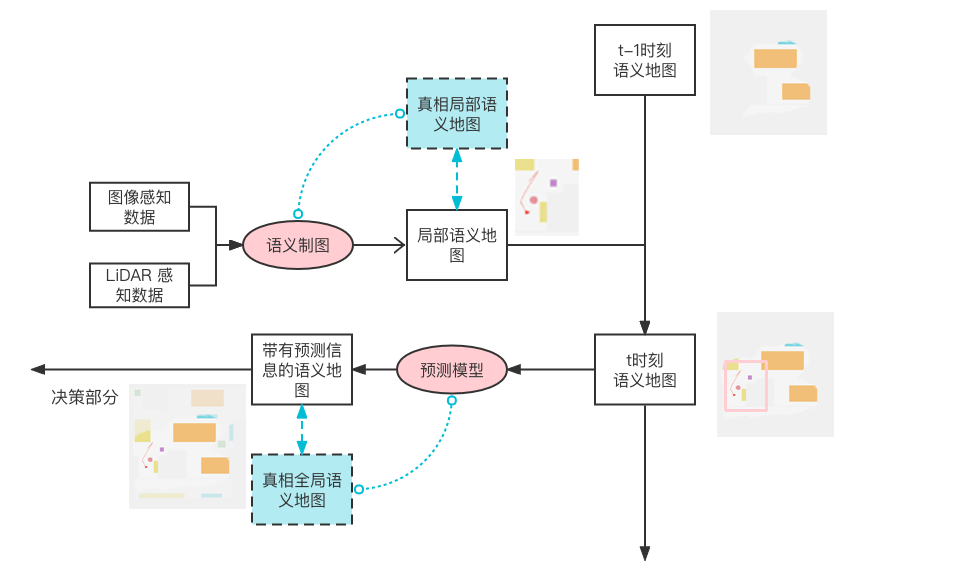
\includegraphics[width=10cm]{assets/perception-example.png}
    \note{
        \begin{itemize}
            \item 感知部分总体上分为两个部分:语义制图和预测模型
            \item 在智能体运行过程中,感知部分将会在每一时刻接收新的传感器数据,在 $t$ 时刻,传感器数据会首先输入语义制图模型,得到关于智能体视野内的局部语义地图。
            \item 得到局部语义地图后,结合上一时刻的已探索语义地图,得到这一时刻更新后的已探索语义地图。注意这一地图是最新的已经探索部分的地图,其中包含各区域中语义目标分布的信息
            \item 当前的已探索语义地图会交给预测模型,对尚未探索的部分进行估计,得到带有预测信息的语义地图,这张地图将会交给决策部分来对长期目标进行规划
        \end{itemize}
    }    
\end{frame}

\begin{frame}{语义制图模型}
    TODO: 图
    \begin{itemize}
        \item 单独训练
        \item 预训练+调优:CMX \cite{cmx}
    \end{itemize}
    \note{
        对于语义制图模型,我们仿照参考文献 [16],使用一个语义分割模型,将传感器的 RGB 和深度信息输入其中,得到语义分割图像。语义分割图像会被用来和模拟器提供的当前视野的语义分割真相来对比,作为模型的监督。
        
        得到的语义分割会被投射到深度信息给出的点云中,从而确定每一点所属物体的语义。最后从上方观察点云、将语义分布投射到地图上得到局部的语义地图。

        \begin{itemize}
            \item 注意此模型的输入与智能体的行动方式无关,因为它只关心视野中的情况。因此这个模型可以脱离智能体单独训练,也可以采用预训练的大型模型微调。
            \item 我们计划使用结合能够利用 RGB-D 多模态数据的语义分割模型 CMX 在场景下 fine-tune 作为语义制图模型。能够结合 RGB 信息和深度信息进行语义分割也是我们和我们所参考的工作的区别之一。
        \end{itemize}
    }
\end{frame}

\begin{frame}{预测模型}
    TODO: 图
    \note{
        对于预测模型,我们从模拟器获得真相的全局语义地图作为监督信息,鼓励模型输出的预测结果贴近真实。
        \begin{itemize}
            \item 这一部分处理了语义目标导航任务中,对语义先验的需求。
            \item 由于预测模型的输入——最新时刻的已探索语义地图与智能体的行动方式有关,所以我们令其与智能体同时进行训练。因为我们对预测的显式建模、将其与强化学习部分分离,所以这种训练是通过梯度优化进行的。
            \item 与我们参考的论文 [16] 相比,他们对语义先验的处理方式是将其集成在全局策略器中,然后用强化学习的方法训练。而我们将其使用全监督的方式实现,我们期待这样能让预测结果更好,并且由于使用梯度优化,收敛速度更快。
            \item 对于真相的获取:如果模拟器能够提供真相的语义地图,那么万事大吉。如果模拟器不能提供真相的语义地图,我们认为可以利用前一个语义制图模块,在训练开始前让其在地图中游走绘制真相。
        \end{itemize}
    }
\end{frame}